\documentclass[12pt]{article}
\usepackage{amsmath, amssymb, amsthm, bm}
\usepackage{geometry}
\usepackage{tikz}
\usetikzlibrary{arrows.meta, calc, positioning}
\usepackage{xcolor} 
\usepackage[skip=0.8em]{parskip}

\newtheorem{proposition}{Proposition}
\newtheorem{theorem}{Theorem}
\newtheorem{lemma}{Lemma}
\theoremstyle{definition}
    \newtheorem{definition}{Definition}[section]
    \newtheorem{condition}{Condition}
\theoremstyle{remark}
    \newtheorem{remark}{Remark}[section]

\geometry{margin=1in}

\begin{document}

\section*{Basic Setup: Admissibility in the Normal Experiment}

Let $X \in \mathbf{R}^k$ denote a random vector distributed according to a multivariate normal distribution with mean $\mu$ and known, invertible covariance matrix $\Sigma$, that is,
\[
X \sim N(\mu, \Sigma), \quad \mu \in \Lambda \equiv \mathbf{R}^k, \; \Sigma > 0.
\]

We are interested in testing the composite null hypothesis
\begin{equation} \label{eq:null}
H_0 : \mu \in \Lambda_0 \quad \text{versus} \quad H_1 : \mu \in \Lambda_1 = \Lambda \setminus \Lambda_0,
\end{equation}
where
\[
\Lambda_0 = \{ \mu \in \Lambda : \mu \le 0 \}, \qquad \Lambda_1 = \{ \mu \in \Lambda : \mu_j > 0 \text{ for some } j \}.
\]

A test is a measurable function $\phi : \mathbf{R}^k \to [0,1]$, where $\phi(x)$ denotes the probability of rejecting $H_0$ given observation $x$.  The test $\phi$ satisfies the finite-sample size constraint
\begin{equation} \label{eq:size}
\sup_{\mu \in \Lambda_0} E_\mu[\phi(X)] \leq \alpha,
\end{equation}
for some pre-specified level $\alpha \in (0,1)$.

Because the sample mean $\bar X$ is a sufficient statistic for $\mu$ when the data are i.i.d. normal, we may, without loss of generality, set $n=1$ and work directly with the single observation $X$.

It is well known that there is no uniformly most powerful (UMP) test for \eqref{eq:null}.  Instead, one can study admissibility of tests satisfying \eqref{eq:size}.  Following Romano and Shaikh (2015), a test $\phi$ satisfying \eqref{eq:size} is:
\begin{itemize}
    \item \emph{$\alpha$-admissible} if for any other test $\tilde \phi$ satisfying \eqref{eq:size},
    \[
    E_\mu[\tilde \phi] \ge E_\mu[\phi] \text{ for all } \mu \in \Lambda_1
    \quad \Rightarrow \quad
    E_\mu[\tilde \phi] = E_\mu[\phi] \text{ for all } \mu \in \Lambda_1;
    \]
    \item \emph{$d$-admissible} if for any other test $\tilde \phi$ satisfying \eqref{eq:size},
    \[
    E_\mu[\tilde \phi] \ge E_\mu[\phi] \text{ for all } \mu \in \Lambda_1, \quad
    E_\mu[\tilde \phi] \le E_\mu[\phi] \text{ for all } \mu \in \Lambda_0
    \quad \Rightarrow \quad
    E_\mu[\tilde \phi] = E_\mu[\phi] \text{ for all } \mu \in \Lambda.
    \]
\end{itemize}

Romano and Shaikh (2015) show that any test $\phi$ satisfying \eqref{eq:size} whose acceptance region is a closed, convex subset of $\mathbf{R}^k$ containing $\Lambda_0$ is $d$-admissible.  If, in addition, the supremum in \eqref{eq:size} is attained and the inequality holds with equality, then $\phi$ is also $\alpha$-admissible. However, there is no circulating paper so we cannot cite and so I decided to prove this result here as a preliminary result for the case that is relevant for our paper. 

\newpage 

\section*{The unrestricted case in the Normal location model}

\subsubsection*{The Equivalence Theorem}

\begin{theorem}[Admissibility–Convexity Equivalence]
\label{thm:admissibility-convexity}
Let $X \sim N(\mu,\Sigma)$, where $\Sigma$ is known and positive definite and
$\mu \in \mathbf{R}^k$.
Consider testing
\[
H_0 : \mu \in \Lambda_0 = \{\mu \le 0\}
\quad \text{versus} \quad
H_1 : \mu \in \Lambda_1 = \mathbf{R}^k \setminus \Lambda_0.
\]
Let $\phi$ be a nonrandomized test satisfying the size constraint
\[
\sup_{\mu \in \Lambda_0} E_\mu[\phi(X)] \le \alpha,
\]
and denote its acceptance region by
$A_\phi = \{x \in \mathbf{R}^k : \phi(x) = 0\}$.
Then $\phi$ is admissible if and only if $A_\phi$ is closed and convex.
\end{theorem}

\begin{proof}
Since the normal location family belongs to the class of exponential families, the result follows as a specialization of Theorem~6.7.1 and Corollary~6.7.1 in Lehmann and Romano (2005, Section~6.7). For completeness, we outline the argument.

Write the normal density in canonical exponential-family form
\[
f(x;\mu)=(2\pi)^{-k/2}|\Sigma|^{-1/2}
\exp\Big\{\theta'x - A(\theta)\Big\},
\qquad A(\theta)=\tfrac12\,\mu'\Sigma^{-1}\mu ,\qquad \theta'=\mu'\Sigma^{-1},
\]
so the sufficient statistic is $T(x)=x$ and the canonical parameter is $\theta=\Sigma^{-1}\mu$. Since $\Sigma$ is fixed and invertible, the mapping $\mu \mapsto \theta$ is one-to-one, and it is convenient to express all arguments directly in terms of $\mu$.

\noindent\emph{Sufficiency.}
If $A_\phi$ is closed and convex, Theorem~6.7.1 and Corollary~6.7.1 of Lehmann and Romano (2005) imply that $\phi$ is admissible (and $\alpha$–admissible when the supremum in the size constraint is attained) provided that the following regularity condition holds: 
\begin{condition}[Regularity Condition]\label{cond:LH-67regularity}
If $ A_\phi\cap\{x:a'x>c\}=\emptyset$ for some $c>0$, then there exists $ \mu^*\in \mathbf R^k$ and a sequence $\lambda \to \infty$ such that $\mu_{\lambda} := \mu^* + \lambda a \in \Lambda_1$.
\end{condition}


In the normal location family, this condition is automatically satisfied because the parameter space for $\mu$ is unconstrained (i.e., $\Lambda = \mathbf R^k$). The premise of the condition, $A_\phi\cap\{x:a'x>c\}=\emptyset$, restricts the vector $a$ to directions along which $A_\phi$ is bounded. That is, it implies $A_\phi \subseteq \{x: a'x \le c\}$.

Note that $\Lambda_1$ includes all vectors with at least one positive component ($\mu_j > 0$ for some $j\in \{1,\dots,k\}$). Let $a \in \mathbf{R}^k$ be a nonzero vector and $\mu^* \in \mathbf{R}^k$ be any point (for instance, $\mu^* = 0$). Consider the ray $\mu_{\lambda} = \lambda a$. As $\lambda \to \infty$, the vector $\mu_{\lambda}$ diverges in the direction of $a$. We need to consider two cases: 
\begin{itemize}
    \item $a\in \Lambda_1$: If the direction vector $a$ has at least one positive component ($a_j > 0$ for some $j$), then the $j$-th component of $\mu_{\lambda}$ is positive, implying $\mu_{\lambda} \in \Lambda_1$.
    \item $a\in \Lambda_0$: If $a$ has only nonpositive components ($a_j \le 0$ for all $j$), then $A_\phi\cap\{x:a'x>c\}\ne \emptyset$, so the premise of Condition~\ref{cond:LH-67regularity} fails and the condition is vacuously satisfied.
\end{itemize}
Therefore, in the normal location model, Condition~\ref{cond:LH-67regularity} always holds. For any bounded half-space disjoint from the convex $A_\phi$, the corresponding ray $\mu^*+\lambda a$ necessarily points into $\Lambda_1$ for large $\lambda$, unless $A_\phi$ is itself unbounded in that direction. Since $\Lambda_0$ occupies only one closed orthant, every other direction eventually exits into $\Lambda_1$. Hence the regularity condition is satisfied, and Theorem~6.7.1 applies. See Figure \ref{fig:ray} for a graphical illustration. 

\noindent\emph{Necessity.}


\begin{figure}[h!]
\centering
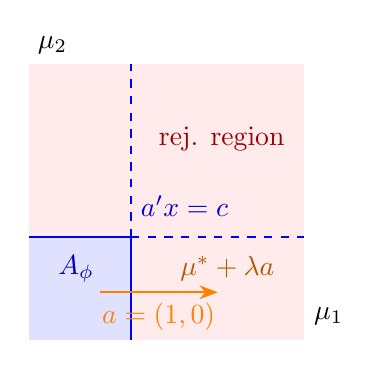
\begin{tikzpicture}[scale=1,>=Stealth]

% axes
\draw[->] (-0.3,0) -- (3.2,0) node[right] {$\mu_1$};
\draw[->] (0,-0.3) -- (0,3.2) node[above] {$\mu_2$};

% (red) rejection background over the whole plotting window
\fill[red!8] (-0.3,-0.3) rectangle (3.2,3.2);

% acceptance region A_phi: {max(x1,x2) <= 1} = square [<=1, <=1]
\fill[blue!12] (-0.3,-0.3) rectangle (1,1);
\draw[blue,thick] (1,-0.3) -- (1,1);
\draw[blue,thick] (-0.3,1) -- (1,1);

% helpful dashed extensions of the boundaries
\draw[blue,thick,dashed] (1,1) -- (1,3.2);
\draw[blue,thick,dashed] (1,1) -- (3.2,1);

% labels
\node[blue!70!black] at (0.3,0.6) {$A_\phi$};
\node[red!60!black] at (2.15,2.25) {rej. region};
%\node[blue!70!black,anchor=south east] at (1,1) {$(1,1)$};

% example direction a and ray illustrating the condition
\draw[->,thick,orange] (0.6,0.3) -- (2.1,0.3)
  node[midway,below] {$a=(1,0)$};
\node[orange!70!black,anchor=west] at (1.5,0.6) {$\mu^*+\lambda a$};

% annotate the supporting half-space boundary a'x=c when a=(1,0)
\node[blue!80!black,anchor=west] at (1,1.4) {$a'x=c$};

\end{tikzpicture}
\caption{Acceptance region $A_\phi=\{x:\max(x_1,x_2)\le 1\}$ (blue square). 
Everything \emph{outside} the blue region is rejection (light red). 
The dashed lines extend the boundaries $x_1=1$ and $x_2=1$. 
The arrow shows a direction $a=(1,0)$ as used in condition \eqref{cond:LH-67regularity}.}\label{fig:ray}
\end{figure}


\end{proof}


\begin{lemma}\label{lem:odd-ratio}
Let $X\sim N(\mu,\Sigma)$ with positive definite $\Sigma$. Let $\mu_0=0$ and $\mu_1\ne 0$, and set $v=\Sigma^{-1}\mu_1$. 
Let $E\subset\mathbf{R}^d$ be closed, convex, and of positive measure. Fix $t^\star\in\mathbf{R}$ and let $B\subset\mathbf{R}^d$ such that $P_{\mu_0}(B)>0$, $B \subseteq E\cap\{x:\, v^\top x \le t^\star\}$, and $\sup_{x\in E} v^\top x > t^\star$. Then
\[
\frac{P_{\mu_0}(X\in B)}{P_{\mu_1}(X\in B)} > \frac{P_{\mu_0}(X\in E)}{P_{\mu_1}(X\in E)}~.
\]
\end{lemma}

\begin{proof}
Let $f_\mu(x)$ denote the density of $N(\mu, \Sigma)$ and define the likelihood ratio
\[
L(x) = \frac{f_{\mu_1}(x)}{f_{\mu_0}(x)} 
= \exp\!\left(x^\top \Sigma^{-1}\mu_1 - \tfrac{1}{2}\mu_1^\top \Sigma^{-1}\mu_1\right)
= c\, e^{v^\top x}~,
\]
where $c>0$ is a constant. For any measurable set $C$ with $P_{\mu_0}(C) > 0$,
\[
\frac{P_{\mu_1}(X \in C)}{P_{\mu_0}(X \in C)} 
= \frac{\int_C f_{\mu_1}(x)\,dx}{\int_C f_{\mu_0}(x)\,dx}
= \frac{\int_C L(x) f_{\mu_0}(x)\,dx}{P_{\mu_0}(C)}
= E_{\mu_0}[L(X) \mid X \in C]~.
\]
Hence,
\[
\frac{P_{\mu_0}(X \in C)}{P_{\mu_1}(X \in C)} 
= \frac{1}{E_{\mu_0}[L(X) \mid X \in C]}~,
\]
and to establish the stated inequality, it suffices to show that 
$E_{\mu_0}[L(X) \mid X \in E] > E_{\mu_0}[L(X) \mid X \in B]$.

Let $\tau:=v^\top X$. Since $L(X)=c\,e^{\tau}$, we have
\[
E_{\mu_0}[L(X)\mid X\in S]=c\,E_{\mu_0}[e^{\tau}\mid X\in S],\qquad S\in\{E,B\}~.
\]
By construction, $B\subseteq E\cap\{\tau\le t^\star\}$ and $E$ contains an open subset of points with $\tau>t^\star$. Therefore, the conditional distribution of $\tau$ given $X\in E$ first-order stochastically dominates the conditional distribution of $\tau$ given $X\in B$:
for all $t \in\mathbf{R}$,
\[
P_{\mu_0}(\tau>t\mid X\in E) \ge P_{\mu_0}(\tau>t\mid X\in B)~,
\]
with strict inequality for some $t>t^\star$ because $P_{\mu_0}(E\cap\{\tau >t^\star\})>0$. Since $e^{\tau}$ is strictly increasing, this implies
\[
E_{\mu_0}[e^{\tau}\mid X\in E] > E_{\mu_0}[e^{\tau}\mid X\in B].
\]
Multiplying by $c$ yields $E_{\mu_0}[L(X)\mid X\in E]>E_{\mu_0}[L(X)\mid X\in B]$, and taking reciprocals gives the stated probability ratio inequality.
\end{proof}




\newpage 
\section*{Irrelevant Information: A Special Case}

Consider the bivariate case $k = 2$ and impose a restriction on the parameter space:
\[
\Lambda = \{ (\mu_1, \mu_2) \in \mathbf{R}^2 : \mu_2 \le \mu_1 \}.
\]
The null hypothesis remains
\[
H_0 : \mu_1 \le 0, \; \mu_2 \le 0, \qquad H_1 : \text{not both } \mu_j \le 0.
\]

We compare two simple non-randomized tests that both satisfy \eqref{eq:size} at level $\alpha$ but differ in the information they use:

\begin{itemize}
    \item \textbf{Short test:} reject $H_0$ when $\phi_{s} := I\{X_1 > c_s\}=1$ for some critical value $c_s$ chosen to satisfy
    \[
    P_{0}(X_1 > c_s) = \alpha.
    \]

    \item \textbf{Long test:} reject $H_0$ when $\phi_{l} :=I\{\max\{X_1, X_2\} > c_l\}=1$, with $c_l$ chosen so that
    \[
    P_{0}(\max\{X_1, X_2\} > c_l) = \alpha.
    \]
\end{itemize}

The two tests differ in how they use information in $X_2$.  The long test incorporates $X_2$ symmetrically with $X_1$, whereas the short test ignores it.  When the parameter space is restricted to $\mu_2 \le \mu_1$, the relevance of $X_2$ becomes ambiguous: under many alternatives, $X_2$ may contribute little additional power beyond $X_1$.  

\begin{theorem}[Admissibility–Convexity Equivalence (Restricted Space)]
\label{thm:restricted-admissibility-convexity}
Let $X \sim N(\mu,\Sigma)$, where $k=2$ and $\Sigma$ is known and positive definite.
Consider testing 
$$ H_0 : \mu \in \Lambda_0 = \{\mu \in \Lambda : \mu_1 \le 0, \mu_2 \le 0\} \quad \text{versus}\quad  H_1 : \mu \in \Lambda_1 = \Lambda \setminus \Lambda_0~,$$ 
where the parameter space is restricted to $\Lambda = \{\mu \in \mathbf{R}^2 : \mu_2 \le \mu_1\}$.
A nonrandomized test $\phi$ is admissible if and only if its acceptance region $A_\phi$ is closed and convex.
\end{theorem}

\begin{proof}
\emph{Necessity}. The necessity part (admissibility implies $A_\phi$ is closed and convex) follows directly from the argument in the necessity proof for Theorem \ref{thm:admissibility-convexity}. The contradiction argument, based on strict concavity and randomization, holds over the full space $\mathbf{R}^k$, and therefore remains valid when restricted to the cone $\Lambda \subset \mathbf{R}^2$.

\emph{Sufficiency}. Assume the acceptance region $A_\phi$ is closed and convex. This implies that $\phi$ is the acceptance region of a Generalized Bayes test. For $\phi$ to be admissible relative to the restricted space $\Lambda$, we must verify the regularity condition in \eqref{cond:LH-67regularity}. The condition requires that for any direction $a$ supporting the convex set $A_\phi$, a feasible ray must exist in the parameter space $\Lambda$.

Specifically, if $A_\phi\cap\{x:a'x>c\}=\emptyset$, we need to show there exist $\mu^* \in \Lambda$ and a sequence $\lambda_j \to \infty$ such that the ray $\mu^*+\lambda_j a$ remains in $\Lambda$ and eventually enters $\Lambda_1$. This is established by Lemma \ref{lem:feasible-regularity} below. This  confirms that the necessary ray of parameter values exists and remains within the restricted cone $\Lambda$ for any relevant direction $a$.
Since the Generalized Bayes test $\phi$ satisfies the regularity condition on the feasible space $\Lambda$, $\phi$ is \textbf{admissible} relative to $\Lambda$.
\end{proof}

\begin{lemma}[Feasible-direction regularity on $\Lambda$]
\label{lem:feasible-regularity}
Let $\Lambda=\{\mu\in\mathbf R^2:\mu_2\le \mu_1\}$ be the restricted parameter space. Let $A_\phi\subset\mathbf R^2$ be a closed and convex acceptance region such that $A_\phi$ is contained in the half-space defined by $a'x \le c$ for some vector $a \in \mathbf{R}^2$. If the direction vector $a$ is compatible with the parameter space $\Lambda$ (i.e., its direction does not immediately exit the cone $\Lambda$),
then there exist $\mu^*\in\Lambda$ and a sequence $\lambda_j\to\infty$ such that the ray $\mu^*+\lambda_j a$ belongs to the alternative $\Lambda_1 = \Lambda \setminus \Lambda_0$ for sufficiently large $j$.
\end{lemma}

\begin{proof}
Let $a = (a_1, a_2)'$ be the direction vector in the parameter space. Since $a$ is compatible with the parameter space $\Lambda$, we must have $a_1 \ge a_2$. We need to demonstrate that the ray $\mu_{\lambda}= \mu^* + \lambda a$ maintains $\mu_{\lambda} \in \Lambda$ and $\mu_{\lambda} \in \Lambda_1$ for large $\lambda$.

\medskip

\noindent \textbf{Feasibility:} Choose a starting point $\mu^*=(t,t)'$ with $t<0$. This point is deep inside the feasible cone $\Lambda$ and also inside the null hypothesis $\Lambda_0$.
The constraint for $\mu_{\lambda}$ is $\mu_{\lambda,1} \ge \mu_{\lambda,2}$, or:
\[
(t + \lambda a_1) \ge (t + \lambda a_2) \implies \lambda (a_1 - a_2) \ge 0~.
\]
Since $\lambda > 0$, this requires $a_1 \ge a_2$, which is ensured by the assumption that the direction $a$ is compatible with the cone $\Lambda$. It follows that $\mu_{\lambda}\in \Lambda$.\\

\noindent \textbf{Alternative.}
For $\mu_\lambda$ to exit $\Lambda_0$ and enter $\Lambda_1$, we need at least one coordinate to become positive.
If $a_1 > 0$ or $a_2 > 0$, then as $\lambda \to \infty$,
\[
\mu_{\lambda,1} = t + \lambda a_1 \to \infty
\]
and hence $\mu_\lambda \in \Lambda_1$ for sufficiently large~$\lambda$.
If instead $a_1 \le 0$ and $a_2 \le 0$, then the ray $\mu^*+\lambda a$ moves deeper into $\Lambda_0$,
so $A_\phi$ cannot be bounded in such a direction: the half-space
$\{x:a'x>c\}$ necessarily intersects $A_\phi$.
Thus the premise of the regularity condition does not apply in this case,
and the condition is vacuously satisfied.

The regularity condition is satisfied for all directions $a$ relevant to the convexity of $A_\phi$.
\end{proof}

\paragraph{Comment.} I asked ChatGPT is the proof is right (said it is) but also claims that we could prove the result without the lemma by saying this : Consider the restricted parameter space 
$\Lambda = \{\mu \in \mathbf{R}^2 : \mu_2 \le \mu_1\}$,
a closed convex cone in~$\mathbf{R}^2$. Since the normal model is a canonical exponential family with convex natural parameter space, results by Brown (1966, \emph{Annals of Mathematical Statistics}, Theorem~3.1) and Berger (1985, \emph{Statistical Decision Theory and Bayesian Analysis}, Theorem~8.7.2) imply that:

\begin{quote}
For a canonical exponential family, any generalized Bayes rule that is admissible on the full natural parameter space remains admissible when the parameter space is restricted to any closed convex subset.
\end{quote}

Intuitively, restricting the parameter space to a convex subset cannot create a dominating test that did not already exist on the full space: if a test $\tilde{\phi}$ dominated $\phi$ on~$\Lambda$, the same domination would extend to the full parameter space, contradicting the admissibility of~$\phi$ on~$\mathbf{R}^2$.

\textbf{However}: I could not find a reference for those results so I decided to prove the Lemma. 


\newpage 
\begin{proof}[Proof of Necessity in Theorem~\ref{thm:admissibility-convexity}]
Assume that $\phi$ is admissible and suppose, toward a contradiction, that its acceptance region $A_\phi$ is not convex. Since $\phi$ is nonrandomized, $A_\phi = \{x : \phi(x)=0\}$ and $R_\phi = \{x : \phi(x)=1\}$. Nonconvexity implies that there exist points $x_1,x_2 \in A_\phi$ and $\lambda\in(0,1)$ such that
$x_\lambda = \lambda x_1 + (1-\lambda)x_2 \notin A_\phi$.

Let $A_{\tilde{\phi}} = \overline{\operatorname{conv}}(A_\phi)$ be the closed convex hull of $A_\phi$,
and define $\tilde{\phi} = I\{X\in A_{\tilde{\phi}}^c\}$. Since $A_\phi \subsetneq A_{\tilde{\phi}}$, the difference set $D = A_{\tilde{\phi}}\setminus A_\phi$ is nonempty and, 
by Lemma~\ref{lem:positive-measure-D}, has positive Lebesgue measure.
Therefore, for all $\mu \in \mathbf{R}^k$,
\[
E_\mu[\phi(X)] - E_\mu[\tilde{\phi}(X)]
= \int_D f(x;\mu)\,dx
= P_\mu(X\in D) > 0~,
\]
so $\tilde{\phi}$ rejects less often than $\phi$ at every $\mu$. 

Because $A_\phi$ is properly contained in $A_{\tilde{\phi}}$, the separation theorem for convex sets 
implies the existence of a nonzero vector $v \in \mathbf{R}^k$ and a constant $t^\star\in\mathbf{R}$ such that
\[
A_\phi \subseteq \{x: v^\top x \le t^\star\},
\qquad
A_{\tilde{\phi}} \cap \{x: v^\top x > t^\star\} \neq \emptyset.
\]
Define $E = A_{\tilde{\phi}}$ and $B = A_\phi$.
Then $B \subseteq E\cap\{v^\top x \le t^\star\}$,
$E$ is closed and convex with $m(E)>0$, and $\sup_{x\in E}v^\top x > t^\star$.

\medskip
\noindent
\textbf{Step 3: Likelihood ratio ordering under the normal model.}
Let $\mu_0 \in \arg\max_{\mu\in\Lambda_0}E_\mu[\phi(X)]$ be a least favorable null parameter
and choose $\mu_1 \in \Lambda_1$ with $\mu_1-\mu_0 \ne 0$.
Set $v=\Sigma^{-1}(\mu_1-\mu_0)$ as above.
All assumptions of Lemma~\ref{lem:odd-ratio} are then satisfied by $(E,B,v,t^\star)$,
and applying that lemma yields the strict inequality
\begin{equation}\label{eq:ratio-key}
\frac{P_{\mu_0}(X\in B)}{P_{\mu_1}(X\in B)}
>
\frac{P_{\mu_0}(X\in E)}{P_{\mu_1}(X\in E)}.
\end{equation}

\medskip
\noindent
\textbf{Step 4: Construction of a randomized dominating test.}
Define the randomization constant
\[
\rho^*
=\frac{E_{\mu_0}[\phi(X)]-E_{\mu_0}[\tilde{\phi}(X)]}
{1-E_{\mu_0}[\tilde{\phi}(X)]}
=\frac{P_{\mu_0}(D)}{P_{\mu_0}(A_{\tilde{\phi}})} \in (0,1),
\]
and the randomized test
\[
\phi^{**}(x) = \mathbf{1}_{R_{\tilde{\phi}}}(x) + \rho^*\,\mathbf{1}_{A_{\tilde{\phi}}}(x).
\]
By construction,
\[
E_{\mu_0}[\phi^{**}(X)] = E_{\mu_0}[\tilde{\phi}(X)] + \rho^*\,P_{\mu_0}(A_{\tilde{\phi}}) 
= E_{\mu_0}[\phi(X)],
\]
so $\phi^{**}$ satisfies the same size constraint as $\phi$.

For any $\mu_1\in\Lambda_1$, its power difference is
\[
E_{\mu_1}[\phi^{**}(X)] - E_{\mu_1}[\phi(X)]
= P_{\mu_1}(A_{\tilde{\phi}})\!
\left[\frac{P_{\mu_0}(D)}{P_{\mu_0}(A_{\tilde{\phi}})} - \frac{P_{\mu_1}(D)}{P_{\mu_1}(A_{\tilde{\phi}})}\right].
\]
By rewriting \eqref{eq:ratio-key} as
\(
\frac{P_{\mu_0}(D)}{P_{\mu_1}(D)} > \frac{P_{\mu_0}(A_{\tilde{\phi}})}{P_{\mu_1}(A_{\tilde{\phi}})},
\)
the bracketed term is strictly positive, and thus
$E_{\mu_1}[\phi^{**}(X)] > E_{\mu_1}[\phi(X)]$.
Hence $\phi^{**}$ strictly dominates $\phi$, contradicting the admissibility of $\phi$.

\medskip
\noindent
We conclude that the acceptance region $A_\phi$ must be closed and convex.
\end{proof}

\end{document}
